%% ============================================================================= %%
%% 	Universidade Federal do Tocantins, Campus Universitário de Palmas UFT        %%
%% Programa de Pós-Graduação em Modelagem Computacional de Sistemas	PPGMCS       %%
%%    109 Norte Av. NS 15 AlCNO 14 Bala I Sala 4 - Palmas/TO 77.001-090          %%
%%                          GERÊNCIA DE PROJETOS                                 %%
%% 	              Prof. Dr. Patrick Letouzé Moreira     (letouze@uft.edu.br)     %%
%% 	                        André Barcelos Silva        (barcelos@uft.edu.br)    %%
%% 	                        Denis da Silva Passos       (denispassos@uft.edu.br) %%
%% ============================================================================= %%
%% Antes de compilar este template pela primeira vez, verifique se o editor está %%
%% apto a compilar arquivo bibtex. No Texmaker:                                  %%
%%    1 - Clique no menu OPÇÕES -> Configurar o Texmaker;                        %%
%%    2 - No lado esquerdo, aba COMPILAR:                                        %%
%%        2.1 - Opção "PdfLaTeX + Bib(la)tex + PdfLaTeX (x2) + View Pdf"         %%
%% ----------------------------------------------------------------------------- %%

%\documentclass[draftcls,12pt,onecolumn,conference]{IEEEtran}		%% Template Journal IEEE Transactions RASCUNHO
\documentclass[journal]{IEEEtran}									%% Template Journal IEEE Transactions PADRÃO
	%% NÃO É POSSÍVEL UTILIZAR OS DOIS COMANDOS ACIMA SIMULTANEAMENTE.
	%% Ambos comandos \documentclass[]{} formatam o trabalho de acordo com o formato IEEE Transactions.
	%% Para alterar a formatação PADRÃO para a formatação RASCUNHO, basta descomentar um comando 
	%% \documentclass e comentar o outro comando \documentclass utilizando o símbolo % (porcentagem)
	%% a frente para comentar (Comentar significa dizer que tal comando comentado não será utilizado).


%% ________________________________________________________________________________________________
%% Pacotes de comandos do LaTeX
\usepackage{amsmath}			%% Equações matemáticas (American Mathematical Society)
\usepackage{cite}				%% Citações
\usepackage[utf8]{inputenc}		%% Padrão UTF8 - Acentuações e Ç
\usepackage{multirow}			%% Concatenaçao de linhas em tabelas
\ifCLASSINFOpdf
	\usepackage[pdftex]{graphicx}
	\DeclareGraphicsExtensions{.jpg,.jpeg,.png}
\fi

%% ________________________________________________________________________________________________
%% Zona de "hifenização" de palavras 
\hyphenation{pa-la-vra}

%% Título do documento
\title{Título Completo do Projeto}

%% Nomes dos autores (Estudante(s), Orientador(es) e Colaborador(es)), suas filiações e emails
\author{
	\IEEEauthorblockN{Carlos~J.~R.~Chagas\IEEEauthorrefmark{1},}		%% Autor 1 e sua filiação {1}
	\IEEEauthorblockN{Oswaldo~G.~Cruz\IEEEauthorrefmark{1},}			%% Autor 2 e sua filiação {1}
	\IEEEauthorblockN{Cesare~M.~G.~Lattes\IEEEauthorrefmark{2}}\\		%% Autor 3 e sua filiação {2}
	\IEEEauthorblockA{\IEEEauthorrefmark{1}Universidade~Federal~do~Rio~de~Janeiro,~Brasil\\	%% Filiação 1
		\{cchagas, gcruz\}@ufrj.edu.br}\\								%% Emails dos autores 1 e 2
	\IEEEauthorblockA{\IEEEauthorrefmark{2}Centro~Brasileiro~de~Pesquisas~Físicas\\			%% Filiação 2
		lattes@cbpf.br}													%% Email do autor 3
}

	%% O símbolo ~ (til) entre os nomes auxilia na centraliação das palavras.
	%% O comando \\ (contrabarra contrabarra) é utilizado para quebrar linha
	%% Utiliza-se o comando \ (contrabarra) para imprimir caractéres especiais do LaTeX ao texto.
	%% Caractéres especiais: $ # % ^ & _ { } ~
	%% Para imprimir \ ao texto, utiliza-se o comando: $\backslash$.

%% ________________________________________________________________________________________________
%% Início do trabalho
\begin{document}

\markboth{Gerência~de~Projetos,~Vol.~1,~No.~1,~Novembro~2016}{}		%% Cabeçalho de versão do trabalho

\maketitle 	%% Zona de criação do título e autores no arquivo final

%% ________________________________________________________________________________________________
%% Abstract (Resumo, em português)
\begin{abstract}
O texto do seu resumo vai aqui.
\end{abstract}

%% Palavras-chave
\begin{IEEEkeywords}
máximo cinco, mínimo três, ordem alfabética, palavras minusculas, termos compostos
\end{IEEEkeywords}

%% ________________________________________________________________________________________________
\section{Introdução}
\IEEEPARstart{P}{rimeira} palavra da introdução deve ser escrita de acordo com o comando "IEEEPARstart".

Modelo de citação de trabalhos externos \cite{Pmi2008}. Assim como \cite{Kahale2008}.	%% Vide referências no arquivo "referencias.bib".

\subsection{Objetivo Geral}
Seu texto vai aqui.

\subsection{Objetivos Específicos}
Modelo de listagem de itens:

\begin{itemize}
\item Primeiro item da lista;
\item Segundo item da lista;
\item Penúltimo item da lista;
\item Último item da lista.
\end{itemize}

%% ________________________________________________________________________________________________
\section{Metodologia}
Seu texto vai aqui.

\subsection{Materiais}
Exemplo de utilização de equação matemática junto ao texto entre \$ simples, onde $x=\frac{-b\pm\sqrt{b^2-4ac}}{2a}$.

\subsection{Ferramentas}
Exemplo de utilização de equação matemática projetada, entre \$\$ duplos:

$$\left|{1\over N}\sum_{n=1}^N \gamma(u_n)-{1\over 2\pi}\int_0^{2\pi}\gamma(t){\rm d}t\right| \le {\varepsilon\over 3}.$$

\subsection{Métodos}
Exemplo de uma matriz quadrada de 3 posições:
$$\begin{bmatrix}
	0 & 1 & 2 \\ 
	1 & 2 & 3 \\ 
	2 & 3 & 4
\end{bmatrix}$$

Exemplo de equação matemática de múltiplas camadas:

	\begin{eqnarray}
		x & = & m + n + p	\nonumber\\ %% Retira a contagem de linhas da equação
		y&=&z + w + u		\\ 			%% Apenas quebra de linha com enumeração
		x& &p+n							%% 
	\end{eqnarray}

\subsection{Processos}

Modelo de tabela. Vide Tabela \ref{t:modelo}.

\begin{table}[h] 
	\centering
	\caption{Legenda da Tabela Modelo.}
	\begin{tabular}{l|cr}
		\hline
			{\bf Sexo} & {\bf UF} & {\bf Idade}\\
		\hline
			M  & PR & 41 \\
			F  & TO & 63 \\
		\hline
			{\bf TOTAL} & {\bf 02} & {\bf 104}\\
		\hline
		\end{tabular}
	\label{t:modelo}
\end{table}

	%% O comando \begin{table} inicia a tabela, assim como o comando \end{table} encerra.
	%% A opção [ht]:
		%% h - here (aqui), posicina a tabela o mais próximo possível do texto onde é construída.
		%% t - top (acima).
		%% p - page (página), posiciona em uma página separada.
		%% b - bottom (abaixo).
		%% Pode-se utilizar essas opções simples [h] ou em conjunto [htp].
		%% Utiliza-se ! para tentar forçar o posicionamento desejado [!h] ou [!ht].
		%% Essas opções funcinam como figuras também.
	%% O comando \centering centraliza a tabela.
	%% O comando \caption{Legenda} insere a legenda da tabela.
	%% O comando \begin{tabular} inicia a tabulação (colunas).
	%% As opções {l|cr}:
		%% A quantidade de letras representa a quantidade de colunas.
		%% Cada letra significa a orientação dos dados na coluna.
		%% l - left (esquerda).
		%% c - center (centro).
		%% r - right (direita).
		%% O símbolo | imprimi linha separadora de colunas. Se não quiser separador, basta apagar o símbolo.
	%% O comando \hline cria linhas horizontais para separar as linhas da tabela.
	%% O símbolo & separa os dados em suas respectivas colunas e o símbolo \\ faz a quebra de linha dos dados.
	%% O comando \label{t:modelo} é um rotulador de figuras e tabelas, utilizado para referenciá-las (\ref{t:modelo}). 


\subsection{Estrutura Analítica do Projeto}
Inserindo figura localmente. É interessante observar que as figuras, além de possuírem uma escala para melhor visualização das informações nelas contidas, precisa ser corretamente determinada a sua localiação, por exemplo, caso cria-se um diretório IMG para guardar as figuras, o caminho correto será \{IMG/grafico.jpg\}.

Vide Figura \ref{f:grafico} sendo referenciada no texto.

%% Modelo de Figura
\begin{figure}[h]
	\centering
	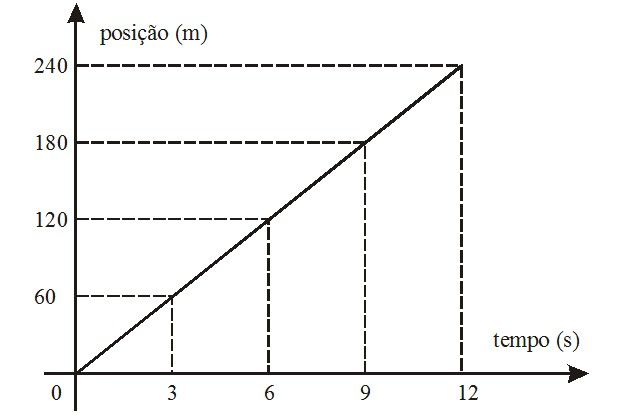
\includegraphics[scale=0.4]{grafico.jpg}
	\caption{Modelo de inserção de figura no LaTeX}
	\label{f:grafico}
\end{figure}

	%% O comando \begin{figure} inicializa a figura, assim como o comando \end{figure} encerra.
	%% O comando \centering centraliza a figura.
	%% O comando 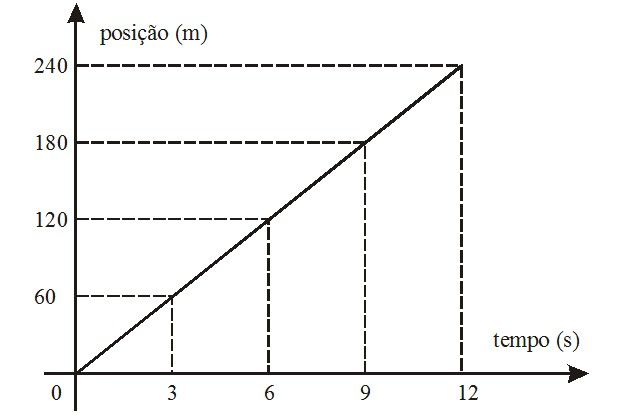
\includegraphics[scale=0.4]{grafico.jpg} adiciona a figura grafico.jpg com escala de 40% (0.4).
	%% O comando \caption{Legenda} insere a legenda da figura.
	%% O comando \label{f:grafico} é um rotulador de figuras e tabelas, utilizado para referenciá-las (\ref{f:grafico}). 

\subsection{Stakeholders}
Seu texto vai aqui.

%% ________________________________________________________________________________________________
\section{Resultados Esperados}
Seu texto vai aqui.

\subsection{Disciplinas Existentes}
Seu texto vai aqui, vide Table \ref{t:disciplinas}.

%% Modelo de Tabela para as Disciplinas Existentes. Inserindo tabela localment.
\begin{table}[h]
\centering
\caption{Disciplinas Existentes.}
\begin{tabular}{l|c|c|c}
  \hline
    {\bf DISCIPLINAS EXISTENTES} & {\bf O} & {\bf S} & {\bf C}  \\ \hline
      Fundamentos de Modelagem Computacional        &   & * & 4 \\ \hline
      Gerência de Projetos                          & * &   & 4 \\ \hline
      Metodologia de Pesquisa                       & * &   & 4 \\ \hline
      Seminários                                    &   & * & 2 \\ \hline
      \multicolumn{4}{l}{{\bf O} - Obrigratórias;}		\\
      \multicolumn{4}{l}{{\bf S} - Sugeridas;}			\\
      \multicolumn{4}{l}{{\bf C} - Créditos. }			\\ \cline{1-4}
\end{tabular}
\label{t:disciplinas}
\end{table}

\subsection{Escopo}
Seu texto vai aqui.

\subsection{Cronograma Esperado}
Seu texto vai aqui. Vide Table \ref{t:cronograma}.

	%% Inserindo código da tabela a partir de um arquivo .tex externo
	%% Modelo de Tabela para o Cronograma Esperado
%% Inserindo tabela em espaço proporcional com o *
\begin{table*}[!ht]
	\centering
	\caption{Cronograma Esperado}
	\begin{tabular}{|r l|c|c|c|c|c|c|c|c|c|c|c|c|} \hline
		\multirow{2}{*}{}& \multirow{2}{*}{}	& \multicolumn{3}{c|}{2016}	& \multicolumn{9}{c|}{2017}   				\\ \cline{3-14}
				&   							& Out & Nov & Dez & Jan & Fev & Mar & Abr & Mai & Jun & Jul & Ago & Set \\ \hline
		I		& Atividade 					& *  & *  & *  &    &    &    &    &    &    &    &    &    			\\ \hline
		II		& Atividade 					&    &    &    & *  & *  & *  &    &    &    &    &    &    			\\ \hline
		III		& Atividade 					&    &    &    &    &    &    & *  & *  & *  & *  &    &    			\\ \hline
		IV		& Atividade 					&    &    &    &    &    &    &    &    &    & *  & *  & *  			\\ \hline
	\end{tabular}
	\label{t:cronograma}
\end{table*}
	
	%% Comando \input{arquivo.tex} adiciona trechos de código, inclusive textos,
	%% dentro do arquivo principal.
	%% Apenas o arquivo principal deve ser compilado

%% ________________________________________________________________________________________________
\section{Discussão}
Seu texto vai aqui.

\subsection{Riscos Inerentes ao Projeto}
Seu texto vai aqui.

\subsection{Desafios}
Seu texto vai aqui.

\subsection{Oportunidades}
Seu texto vai aqui.

%% ________________________________________________________________________________________________
\newpage 		%% Para interromper a quebra de página, basta comentar o comando: %\newpage
\appendices 	%% Apêndice: Termo de Ciência e Concordância do Orientador

\section*{Termo de Ciência e\\Concordância do Orientador} %% O símbolo * (asterísco) retira a seção da numeração
Declaro estar ciente do teor deste projeto de pesquisa desenvolvido na disciplina de Gerência de Projetos do Programa de Pós-Graduação em Modelagem Computacional de Sistemas da Universidade Federal do Tocantins e considero-o, em princípio, factível.

\vspace{1cm}		%% Espaçamento vertical

\begin{flushright}
Palmas, \_\_\_\_\_ de \_\_\_\_\_\_\_\_\_\_\_\_\_\_\_ de 2017.
\end{flushright}

\vspace{2cm}

\begin{center}
\_\_\_\_\_\_\_\_\_\_\_\_\_\_\_\_\_\_\_\_\_\_\_\_\_\_\_\_ \\
Prof. Dr. Oswaldo~Gonçalves~Cruz\\
Orientador\\
\end{center}

\vspace{1.5cm}

\begin{center}
\_\_\_\_\_\_\_\_\_\_\_\_\_\_\_\_\_\_\_\_\_\_\_\_\_\_\_\_ \\
Carlos~Justiniano~Ribeiro~Chagas\\
Orientando (Proponente)\\
\end{center}

\vspace{1.5cm}

\begin{center}
\_\_\_\_\_\_\_\_\_\_\_\_\_\_\_\_\_\_\_\_\_\_\_\_\_\_\_\_ \\
Prof. Dr. Cesare~Mnasueto~Giulio~Lattes\\
Professor da disciplina de Gerência de Projetos
\end{center}

%% ________________________________________________________________________________________________
\newpage %% Para interromper a quebra de linhas, basta comentar o comando: % \newpage

\bibliographystyle{IEEEtran}	%% Modelo de referências do IEEE Transactions
\bibliography{Referencias}		%% Carregando arquivo "Referencias.bib"

%% ________________________________________________________________________________________________
\newpage %% Para interromper a quebra de linhas, basta comentar o comando: % \newpage


\begin{IEEEbiography}
[{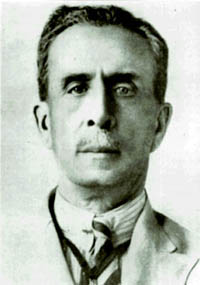
\includegraphics[width=1in,height=1.25in,clip,keepaspectratio]{chagas.jpg}}]{Carlos Justiniano Ribeiro Chagas}
Foi médico, cientista, pesquisador e sanitarista brasileiro. Dedicou-se ao estudo das doenças tropicais. Descobriu o protozoário do gênero Plasmodium, causador da Malária. Descobriu também o parasita Tripanosoma Cruzi, transmissor da doença de Chagas (1879-1934).
\end{IEEEbiography}

\begin{IEEEbiography}
[{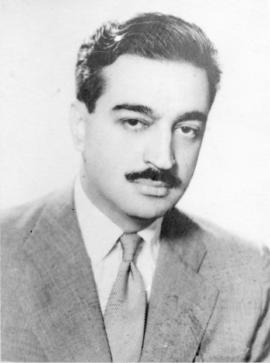
\includegraphics[width=1in,height=1.25in,clip,keepaspectratio]{cruz.jpg}}]{Oswaldo Gonçalves Cruz}
Foi um grande pesquisador que atuou como cientista, médico, bacteriologista, epidemiologista e sanitarista brasileiro. Foi o pioneiro no estudo de doenças tropicais e da medicina experimental no Brasil (1872-1917).
\end{IEEEbiography}

\begin{IEEEbiography}
[{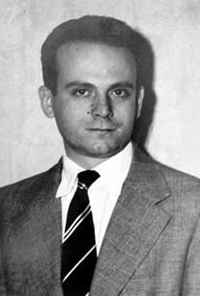
\includegraphics[width=1in,height=1.25in,clip,keepaspectratio]{lattes.png}}]{Cesare Mnasueto Giulio Lattes}
Foi um físico brasileiro, co-descobridor do méson pi, descoberta que levou o Prêmio Nobel de Física de 1950, concedido a Cecil Frank Powell. Fez os seus primeiros estudos em sua cidade natal e depois em São Paulo, vindo a graduar-se na Universidade de São Paulo, formando-se em 1943, em matemática e física (1924-2005).
\end{IEEEbiography}

%% ________________________________________________________________________________________________
\end{document}
%% Fim do Trabalho ================================================================================ %%